% ============================================================
%  ANEXO — Roofline y análisis de bottleneck de kernels NN
%  RECONSTRUIDO: la versión original (rama nn-llm-related-benchmarks) se
%  perdió sin commitear al cambiar de rama. Reconstruido con los números
%  y las 3 figuras regeneradas de nuevo (re-corriendo ci/roofline_suite.py)
%  — coinciden exactamente con los valores originales.
% ------------------------------------------------------------------
\section{Roofline y Análisis de Bottleneck de Kernels NN}
\label{sec:roofline_bottleneck}

\subsection{Contexto}

Evaluación técnica de Vortex como núcleo candidato para el TFG derivado del
de Chacón Alfaro (clúster RISC-V cooperativo para ML). Vortex ya implementa
una jerarquía de caché parametrizable (I\$/D\$ privada, L2 por clúster, L3
global), con coherencia derivada por punto de coherencia (sin snooping),
sobre núcleos \textbf{SIMT} (warps de hilos), no núcleos escalares
independientes. La decisión tomada es aislar un núcleo SIMT de Vortex y
reemplazar su caché por una L1+L2 propia (ver el anexo de implementación
de la L1, rama \texttt{l1\_cache/definition\_and\_interfaces}).

\subsection{Herramienta de medición}

\texttt{ci/roofline\_suite.py} ejecuta los cuatro benchmarks de kernels
neuronales existentes en el repositorio de Vortex --- \texttt{sgemm}
(multiplicación de matrices), \texttt{conv3} (convolución 3$\times$3),
\texttt{softmax} y \texttt{relu} --- bajo una configuración de hardware
compartida, y grafica los cuatro puntos en un mismo diagrama roofline de
FLOP/ciclo contra intensidad aritmética.

\subsection{Línea base: desglose de stalls del pipeline}
\label{ssec:linea_base}

Configuración por defecto: 1 clúster, 1 núcleo, 4 warps, 4 hilos.

\begin{table}[H]
\centering
\caption{Línea base de rendimiento por kernel (warps=4)}
\label{tab:linea_base}
\begin{tabular}{|l|c|c|c|c|c|}
\hline
\textbf{Kernel} & \textbf{Tamaño} & \textbf{Idle scheduler} & \textbf{Stall scrb} & \textbf{IPC} & \textbf{Latencia load} \\
\hline
matmul (sgemm) & -n128   & 58\% & 44\% & 0.417 & 21.7 ciclos \\
conv (conv3)   & -n64    & 61\% & 25\% & 0.393 & 11.6 ciclos \\
softmax        & -n128   & 65\% & 8\%  & 0.354 & 23.3 ciclos \\
relu           & -n65536 & 69\% & 21\% & 0.311 & 22.8 ciclos \\
\hline
\end{tabular}
\end{table}

\begin{figure}[H]
    \centering
    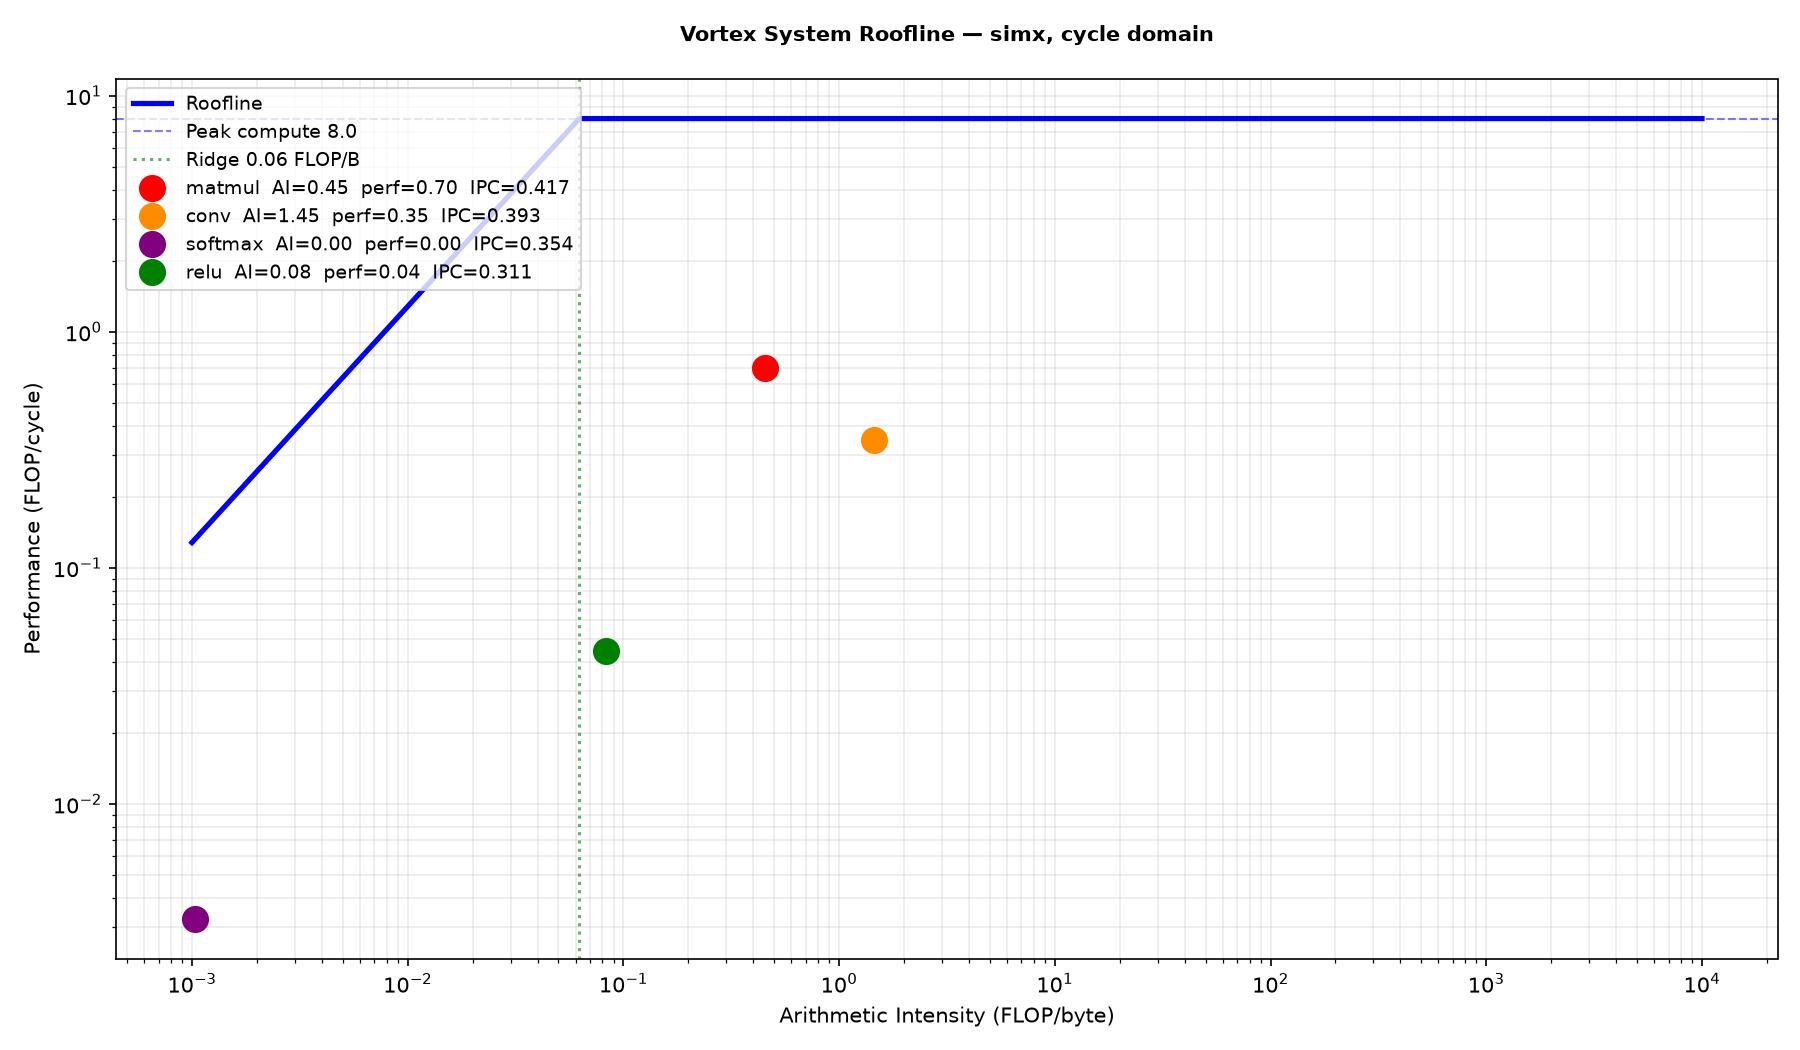
\includegraphics[width=0.85\linewidth]{docs/assets/img/system_roofline.png}
    \caption{Roofline del sistema para los cuatro kernels NN, warps=4 (línea base).}
    \label{fig:roofline_baseline}
\end{figure}

Los cuatro puntos caen muy por debajo tanto del techo de cómputo como de la
línea de ancho de banda de memoria --- ninguno está limitado por FLOPs ni
por ancho de banda. Los contadores de utilización de unidades funcionales
(ALU, FPU, LSU, SFU) están prácticamente en 0\%. El limitador dominante es
el \emph{idle} del planificador (58--69\,\%): la mayoría de los ciclos no
hay ningún warp listo para emitir, con el stall de \emph{scoreboard}
(\texttt{scrb}) como causa visible principal.

\textbf{Causa raíz: ocupancia insuficiente para ocultar latencia.} Con solo
4 warps residentes y latencias de \emph{load} de 12 a 23 ciclos, en cuanto
los 4 warps emiten una operación de latencia larga no queda ningún otro warp
listo para ejecutar, y el núcleo permanece inactivo.

\subsection{Verificación: sensibilidad a la cantidad de warps}

\begin{table}[H]
\centering
\caption{Sensibilidad del IPC a la cantidad de warps}
\label{tab:sensibilidad_warps}
\begin{tabular}{|l|c|c|c|}
\hline
\textbf{Kernel} & \textbf{IPC (warps=4)} & \textbf{IPC (warps=32)} & \textbf{Mejora} \\
\hline
matmul   & 0.417 & 0.919 & 2.2$\times$ \\
conv     & 0.393 & 0.961 & 2.4$\times$ \\
softmax  & 0.354 & 0.740 & 2.1$\times$ \\
relu     & 0.311 & 0.993 & 3.2$\times$ \\
\hline
\end{tabular}
\end{table}

\begin{figure}[H]
    \centering
    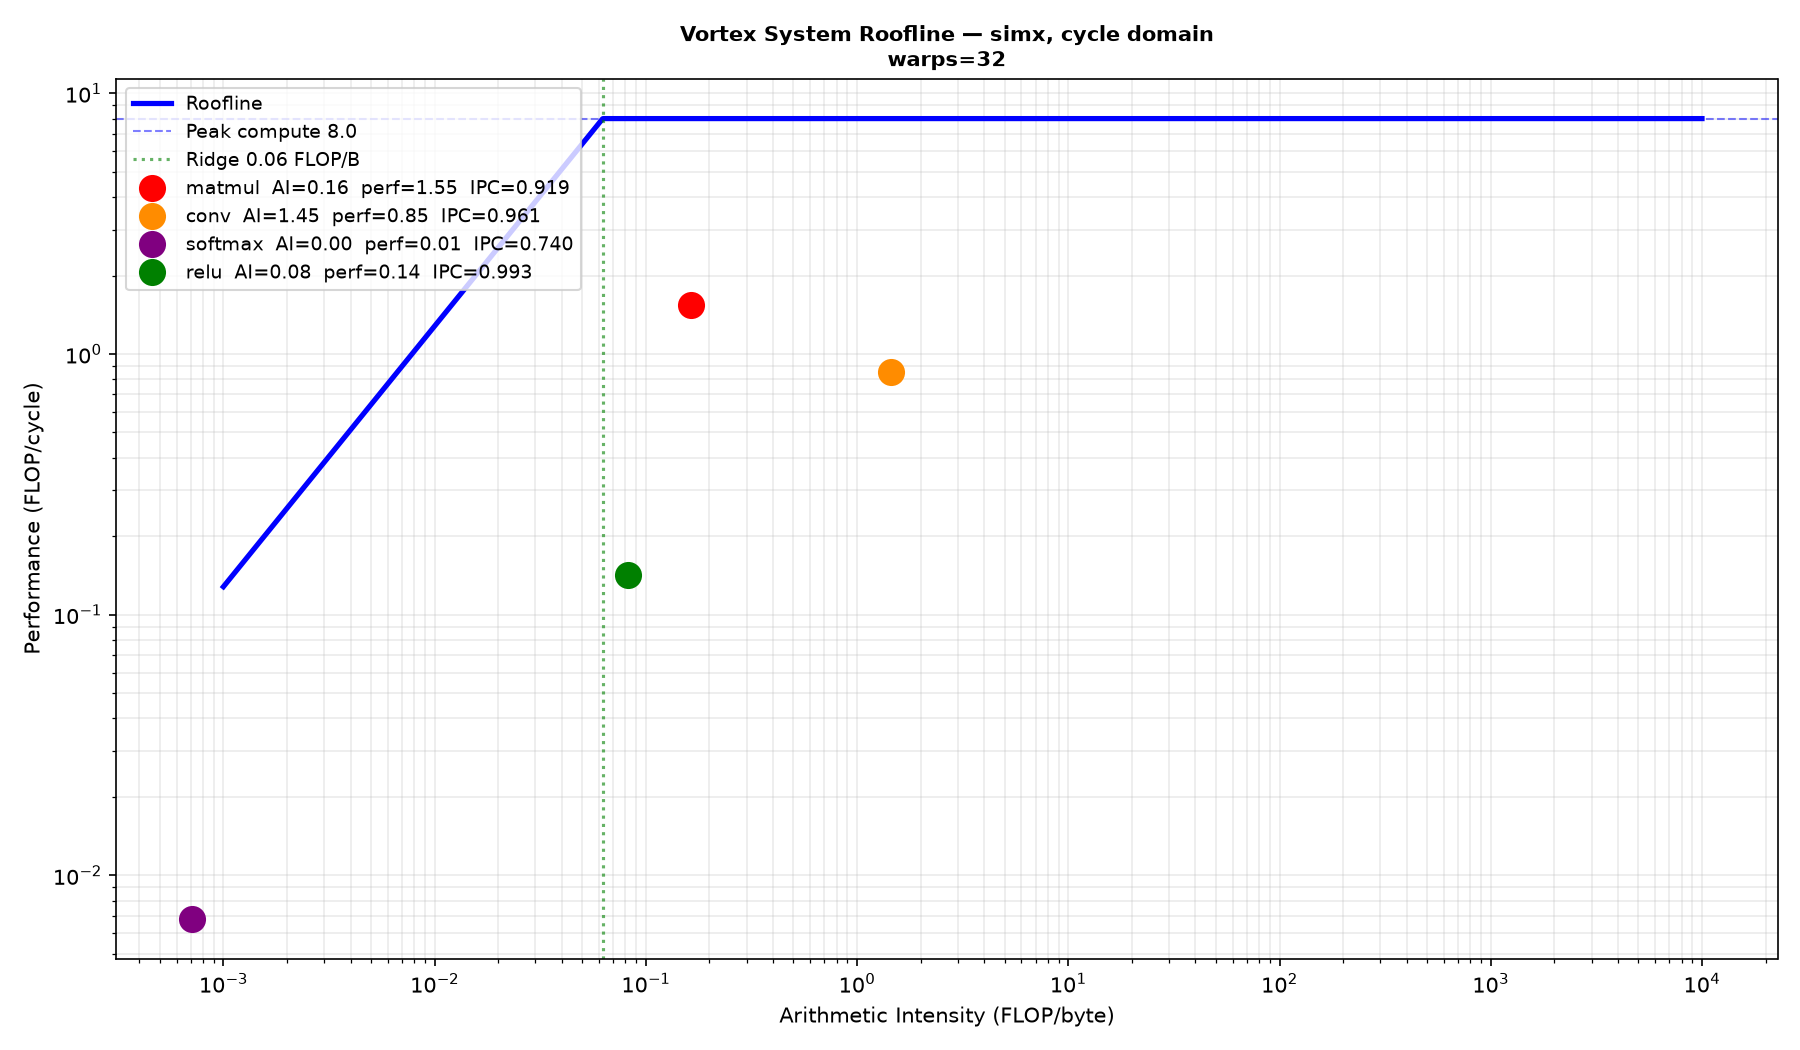
\includegraphics[width=0.85\linewidth]{docs/assets/img/system_roofline_w32.png}
    \caption{Roofline del sistema para los cuatro kernels NN, warps=32.}
    \label{fig:roofline_w32}
\end{figure}

El kernel \texttt{relu} queda casi saturado (idle=1\,\%) --- era puramente
\emph{latency-bound}. El kernel \texttt{softmax} mejora menos (idle=26\,\%
incluso con 32 warps) porque su patrón de tres pasadas sobre los mismos
datos genera más contención de MSHR y de banco (la latencia de
\emph{load} sube a 82 ciclos).

\subsection{Aislar un núcleo}

Configuración \texttt{tinygpu}:

\begin{quote}
\texttt{CONFIGS="-DVX\_CFG\_NUM\_CLUSTERS=1 -DVX\_CFG\_NUM\_CORES=1 \textbackslash \\
\hspace*{1em}-DVX\_CFG\_NUM\_WARPS=2 -DVX\_CFG\_NUM\_THREADS=2 \textbackslash \\
\hspace*{1em}-DVX\_CFG\_ICACHE\_DISABLE -DVX\_CFG\_DCACHE\_DISABLE -DVX\_CFG\_LMEM\_DISABLE"}
\end{quote}

\subsubsection*{Núcleos usados en cada experimento}

Todas las comparaciones de este anexo corren sobre \textbf{un solo
núcleo} (default de Vortex, \texttt{NUM\_CLUSTERS=1, NUM\_CORES=1}, nunca
cambiado):

\begin{table}[H]
\centering
\caption{Núcleos, warps e hilos usados por experimento}
\label{tab:nucleos_experimentos}
\begin{tabular}{|l|c|c|c|c|}
\hline
\textbf{Experimento} & \textbf{Núcleos} & \textbf{Warps} & \textbf{Hilos} & \textbf{Caché} \\
\hline
Línea base (Sec.~\ref{ssec:linea_base}) & 1 & 4 & 4 & con caché \\
Sensibilidad a warps & 1 & 32 & 4 & con caché \\
Núcleo aislado, con caché & 1 & 2 & 2 & con caché \\
Núcleo aislado, sin caché (\texttt{tinygpu}) & 1 & 2 & 2 & sin caché \\
\hline
\end{tabular}
\end{table}

\subsubsection*{Resultado medido: con caché vs. sin caché}

\begin{table}[H]
\centering
\caption{IPC con caché vs. sin caché, mismo núcleo aislado}
\label{tab:con_sin_cache}
\begin{tabular}{|l|c|c|c|c|c|}
\hline
\textbf{Kernel} & \textbf{IPC con caché} & \textbf{IPC sin caché} & \textbf{Caída} & \textbf{ifetch\_lat con} & \textbf{ifetch\_lat sin} \\
\hline
matmul   & 0.214 & 0.076 & 2.8$\times$ & 5.0 ciclos & 22.0 ciclos \\
conv     & 0.201 & 0.077 & 2.6$\times$ & 5.0 ciclos & 21.1 ciclos \\
softmax  & 0.180 & 0.073 & 2.5$\times$ & 5.0 ciclos & 21.2 ciclos \\
relu     & 0.169 & 0.075 & 2.3$\times$ & 5.0 ciclos & 20.5 ciclos \\
\hline
\end{tabular}
\end{table}

Quitar la caché cuesta 2.3--2.8$\times$ de IPC, y el causante principal es
el \textbf{fetch de instrucciones} (5 $\to$ $\sim$21 ciclos sin I\$).

\begin{figure}[H]
    \centering
    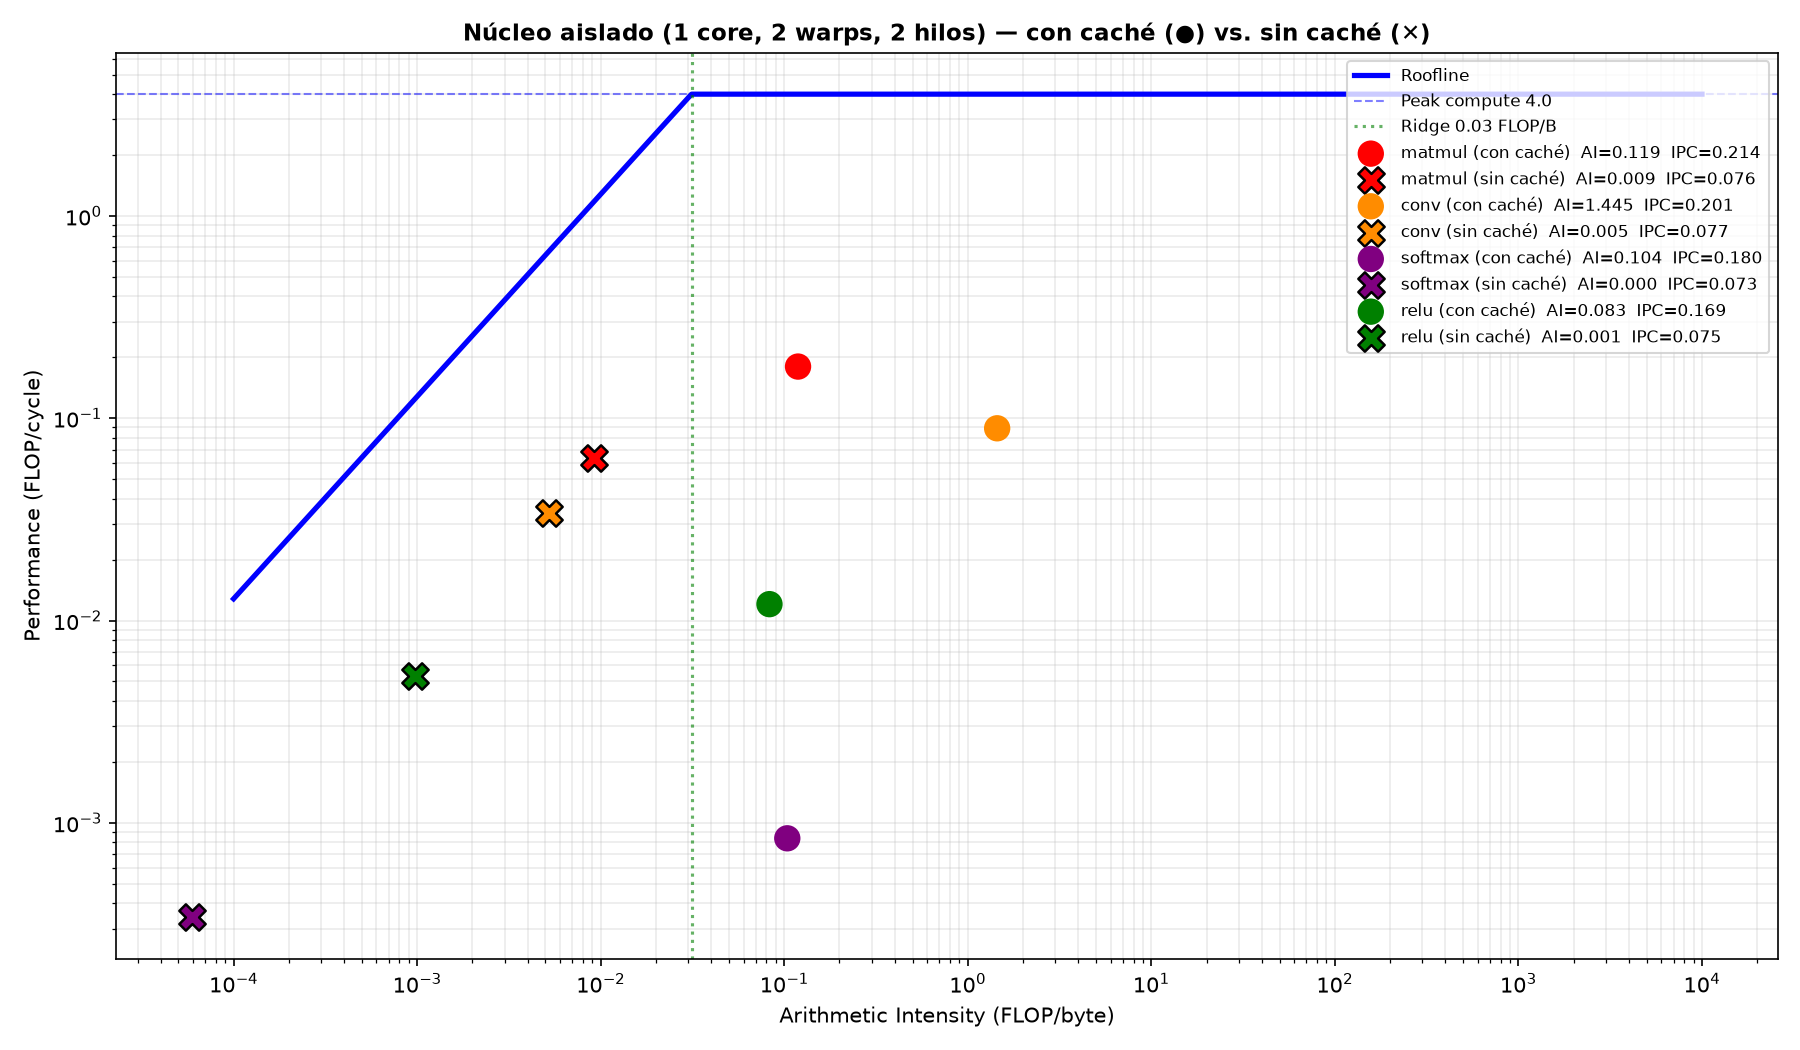
\includegraphics[width=0.85\linewidth]{docs/assets/img/system_roofline_isolated_core.png}
    \caption{Roofline del núcleo aislado, con caché (\textbullet) vs. sin caché ($\times$).}
    \label{fig:roofline_isolated}
\end{figure}

Sin caché, además de rendir menos, la AI también cae 1--2 órdenes de
magnitud (ej. matmul: 0.119 $\to$ 0.009 FLOP/byte).

\subsubsection*{Formato del bus en el punto de aislamiento}

\texttt{VX\_mem\_bus\_if} es un canal valid/ready simple. La divergencia
SIMT ya está resuelta antes de llegar acá: un \texttt{VX\_mem\_coalescer}
funde las peticiones por-hilo del LSU en peticiones más anchas antes de
que salgan del núcleo. Una L1 de reemplazo recibe una petición coalescida
por operación de memoria, no accesos divergentes por hilo.

\subsection{Relación con los objetivos del proyecto}

\begin{table}[H]
\centering
\begin{tabular}{|p{4.2cm}|p{9.3cm}|}
\hline
\textbf{Trabajo realizado} & \textbf{Objetivo / actividad del anteproyecto} \\
\hline
\texttt{roofline\_suite.py} + desglose de stalls &
Instrumentación pedida en OE1 / A-2 / A-3. \\
\hline
Tabla~\ref{tab:linea_base} &
Línea base (A-2) contra la que comparar la L1+L2 nueva en A-22/A-23. \\
\hline
Hallazgo de latencia/ocupancia como limitador dominante &
Insight de diseño para A-3. \\
\hline
Configuración \texttt{tinygpu} &
Punto de partida técnico de A-1. \\
\hline
Formato de \texttt{VX\_mem\_bus\_if} + coalescer &
Resuelve el primer pendiente de A-4. \\
\hline
\end{tabular}
\caption{Mapeo del trabajo de evaluación a los objetivos del anteproyecto}
\label{tab:mapeo_objetivos}
\end{table}

\subsection{Pendientes}

\begin{itemize}
    \item Definir cómo mapear coherencia MESI sobre un solo núcleo aislado.
    \item Separar cuánto de la caída con/sin caché es I\$ vs. D\$.
    \item Experimento con más de un núcleo.
\end{itemize}
